\section{模型的评价与推广}

\subsection{模型的优点}

\begin{enumerate}[label=\textbf{优点 \arabic*}]
	\item \textbf{物理口径唯一，四问横向可比。}附录给定的时间、能耗、充电与链路公式只在公共物理层实现一次（航段几何、载荷—航程、逐段能耗、两阶段充电、链路预算及三态判定），问题一至问题四全部复用，杜绝了"各问各写一套"造成的口径分叉。这是四问结果能够互相印证、层层继承的前提。
	\item \textbf{数值反解严谨且可验证。}最大安全载荷因指数 $3/2$ 无初等反函数，本文用单调性 $+$ Brent 法数值反解并\textbf{强制回代验证}约束紧性，实测相对误差 $5.6\times10^{-15}$，达到了机器精度。工程上"近似公式代替反解"是常见的失分点，本文避免了这一陷阱。
	\item \textbf{结论可证最优而非仅"较优"。}问题一通过 Martello--Toth 型解析下界证明了 18 架次\textbf{在架次数维度上最优}（15 个服务区逐区等于下界）；问题四的分区不可行性是\textbf{精确的图论结论}（连通分量为 1），不含任何启发式近似。这两处使全文有两条"硬结论"支撑。
	\item \textbf{结果可独立复算。}本文用 240 条航段缓存对问题二全部 35 个架次逐段重算，与求解器上报值完全吻合（总能耗均为 83.0100\,kWh），资源占用零冲突、结束时刻自洽偏差小于 0.1\,s。独立的第二套计算显著提升了结果的可信度。
	\item \textbf{敢于报告否定性结论。}对"首批保障时限不可行"与"合法 2/3 组分区不存在"两个问题，本文没有伪造违反约束的方案，而是给出\textbf{定量下界证明}（前 60\,min 最多 8$\sim$10 架次 vs 9 个服务区的 60\,min 需求；单一连通分量）并辅以最小改动方案。这类结论对应急指挥的资源配置具有直接的决策价值。
	\item \textbf{关键结论具备工程指导性。}如"结构载重而非能量才是主导约束"、"中继接入段最弱（116\,dB）故中继应贴近作业空域而非网关"、"分区不省资源也不改善均衡（13/17/21 台·组）"等，均给出了可操作的量化依据。
\end{enumerate}

\subsection{模型的缺点}

\begin{enumerate}[label=\textbf{缺点 \arabic*}]
	\item \textbf{启发式不保证全局最优。}问题二、三的路线规划与中继选址采用构造 $+$ 局部搜索，虽以字典序目标保证了优先级正确、并以独立复算保证了可行性，但无法证明所得路线是全局最优解。
	\item \textbf{连续选址做了充分条件降维。}为规避"连续轨迹 $\times$ 连续三维选址"的最优控制难题，本文采用"存在单一悬停点即可全程覆盖"这一\textbf{充分条件}。该处理保证了只要找到点就必然可行，但可能遗漏"需要多次切换中继位置"的更优方案，因此所得的 30 个中继架次是\textbf{可行上界}而非最优值。
	\item \textbf{时间离散与地形数据引入保守偏差。}$\Delta t=5$\,s 的采样与 30\,m DSM 会使能耗与遮挡判定略偏保守（见 9.4 节），在追求精确能耗评估的场景下需要进一步细化。
	\item \textbf{未考虑动态因素。}模型假定任务期间天气、风场、临时禁飞区与通信干扰恒定，实际救援中这些因素可能显著改变可行域。
\end{enumerate}

\subsection{模型的改进方向}

\begin{enumerate}[label=\textbf{改进 \arabic*}]
	\item \textbf{用精确方法替代启发式。}对问题二的路线与派发，可建立\textbf{混合整数规划}模型并用 CP-SAT 求解小规模实例，或将多目标做 $\varepsilon$-约束处理生成完整 Pareto 前沿，从而给出与启发式解的\textbf{最优性间隙}。
	\item \textbf{把中继选址从充分条件升级为最优控制。}$\Delta t$ 上的选址可形式化为"每时刻可切换中继与悬停点"的动态规划/最短路径问题，允许中继在服务过程中移动，从而降低中继架次数。
	\item \textbf{补齐资源缺口。}问题四显示 $K=1$ 的唯一缺口为 1 组 B 型备用电池。可在模型中把"增配 1 组电池"作为决策变量，评估增配成本与准时率提升的边际效益。
	\item \textbf{引入随机与动态要素。}将需求到达、天气与链路质量建模为随机过程，用滚动时域优化或蒙特卡洛仿真评估方案的鲁棒性，输出"准时率—置信水平"曲线。
	\item \textbf{修正并复核校验器口径。}按 9.3 节的定位结论修订"最早送达时刻"的判据实现，使独立校验器与逐段复算完全一致，形成闭环的质量保证。
\end{enumerate}

\subsection{模型的推广}

本文的模型体系不限于本次设定的山区洪涝场景，可向以下方向推广：

\textbf{（1）其他应急物流场景。}地震、泥石流、雪灾等同样面临"道路中断 $+$ 通信损毁"的复合灾情，本文的"公共物理层 $+$ 四问递进"框架可直接迁移；只需替换 DEM 与节点数据、更新时限分布即可。

\textbf{（2）通信中继的通用选址。}本文"由链路预算反推可达距离、再据此确定选址可行域形状"的方法，适用于任何"接入段与回传段门限不对称"的中继部署问题，如应急通信车、系留气球基站、卫星地面站的选址。

\textbf{（3）异构机队的资源共享调度。}$K$ 组分区实验揭示的"分组丧失规模效应"这一结论，对多基地、多班组的应急资源调度具有普遍意义：\textbf{在资源共享的收益大于独立储备的成本时，应优先集中调度而非分区}。

\textbf{（4）图连通分量方法用于任务划分。}把"必须同组"类硬约束转化为等价关系求连通分量，是处理各类"绑定约束下的分区问题"的通用技巧，可推广至车间班组划分、配送区域划分、检修任务包划分等场景。

\textbf{（5）方法论层面。}"先诊断、再设计"（问题三先证明中继必需，再设计中继方案）与"用解析下界/精确图论给出可证结论"（问题一、四）两条方法论，对数学建模类问题的求解具有普遍借鉴意义。

\section{结论}

本文围绕山区洪涝灾害下的无人机运输与通信协同优化问题，完成了四个问题的建模、求解与验证，主要结论如下：

\begin{enumerate}[label=\textbf{结论 \arabic*}]
	\item 问题一：建立了以"沿线最高点 $+50$\,m"确定巡航海拔、由航程反推巡航能耗的统一物理模型。\textbf{结构载重而非能量是主导约束}（A 型 15/15、B 型 14/15 个服务区受 $Q_{g}$ 约束）。最优组批方案为 \textbf{18 个架次（全 C 型）}，逐服务区等于解析下界、\textbf{可证最优}；总能耗 75.07\,kWh。$\rho_{g}$ 由 0.20 增至 0.35 使架次增至 25，$\rho_{g}\ge0.375$ 时问题开始无可行解。
	\item 问题二：给出 \textbf{35 个架次（全部 B 型）}的多点串飞调度，总能耗 83.01\,kWh、完工 9.78\,h、期望送达准时率 38.8\%。经\textbf{逐段独立复算}，全部架次满足能量预算，资源零冲突，\textbf{物理类硬约束违规 0 条}。并论证\textbf{首批保障时限在本机队下物理不可行}（前 60\,min 至多 4$\sim$6 架次 vs 8 个服务区的 60\,min 需求）。
	\item 问题三：诊断出 \textbf{29/35 个架次存在直连中断}（平均中断占比 31.0\%），证明中继为必需项。给出 \textbf{30 个中继架次}的联合调度，需保障的 29 个架次实现 \textbf{100\% 全程连续通信覆盖}；总能耗 99.68\,kWh，联合完工 9.90\,h。
	\item 问题四：通过连通分量分析证明，在保持问题三安排不变的前提下\textbf{不存在合法的 2 组或 3 组分区}（21 个多点架次把 15 个服务区串成单一连通分量）。定位 3 个桥接架次并给出最小改动方案；资源核算表明\textbf{分区既不省资源也不改善均衡}（K$\,=\,$1/2/3 资源总量 13/17/21，不均衡度 0/1.7718/2.4707），$K=1$ 唯一缺口为 1 组 B 型备用电池。
\end{enumerate}

图~\ref{fig:summary} 汇总了四问的主要指标。可以看到，问题二在引入多点串飞与充电周转后，架次数由问题一的 18 增至 35、能耗由 75.07 升至 83.01\,kWh（$+10.6\%$），并以 2 架 B 型机与 4 组电池完成了 80 箱的全部投送；问题三因新增中继保障使总能耗进一步升至 99.68\,kWh，其中中继仅贡献 16.7\%；问题四则说明在当前架次划分下分区既无收益也不改善均衡。

\begin{figure}[htbp]
	\centering
	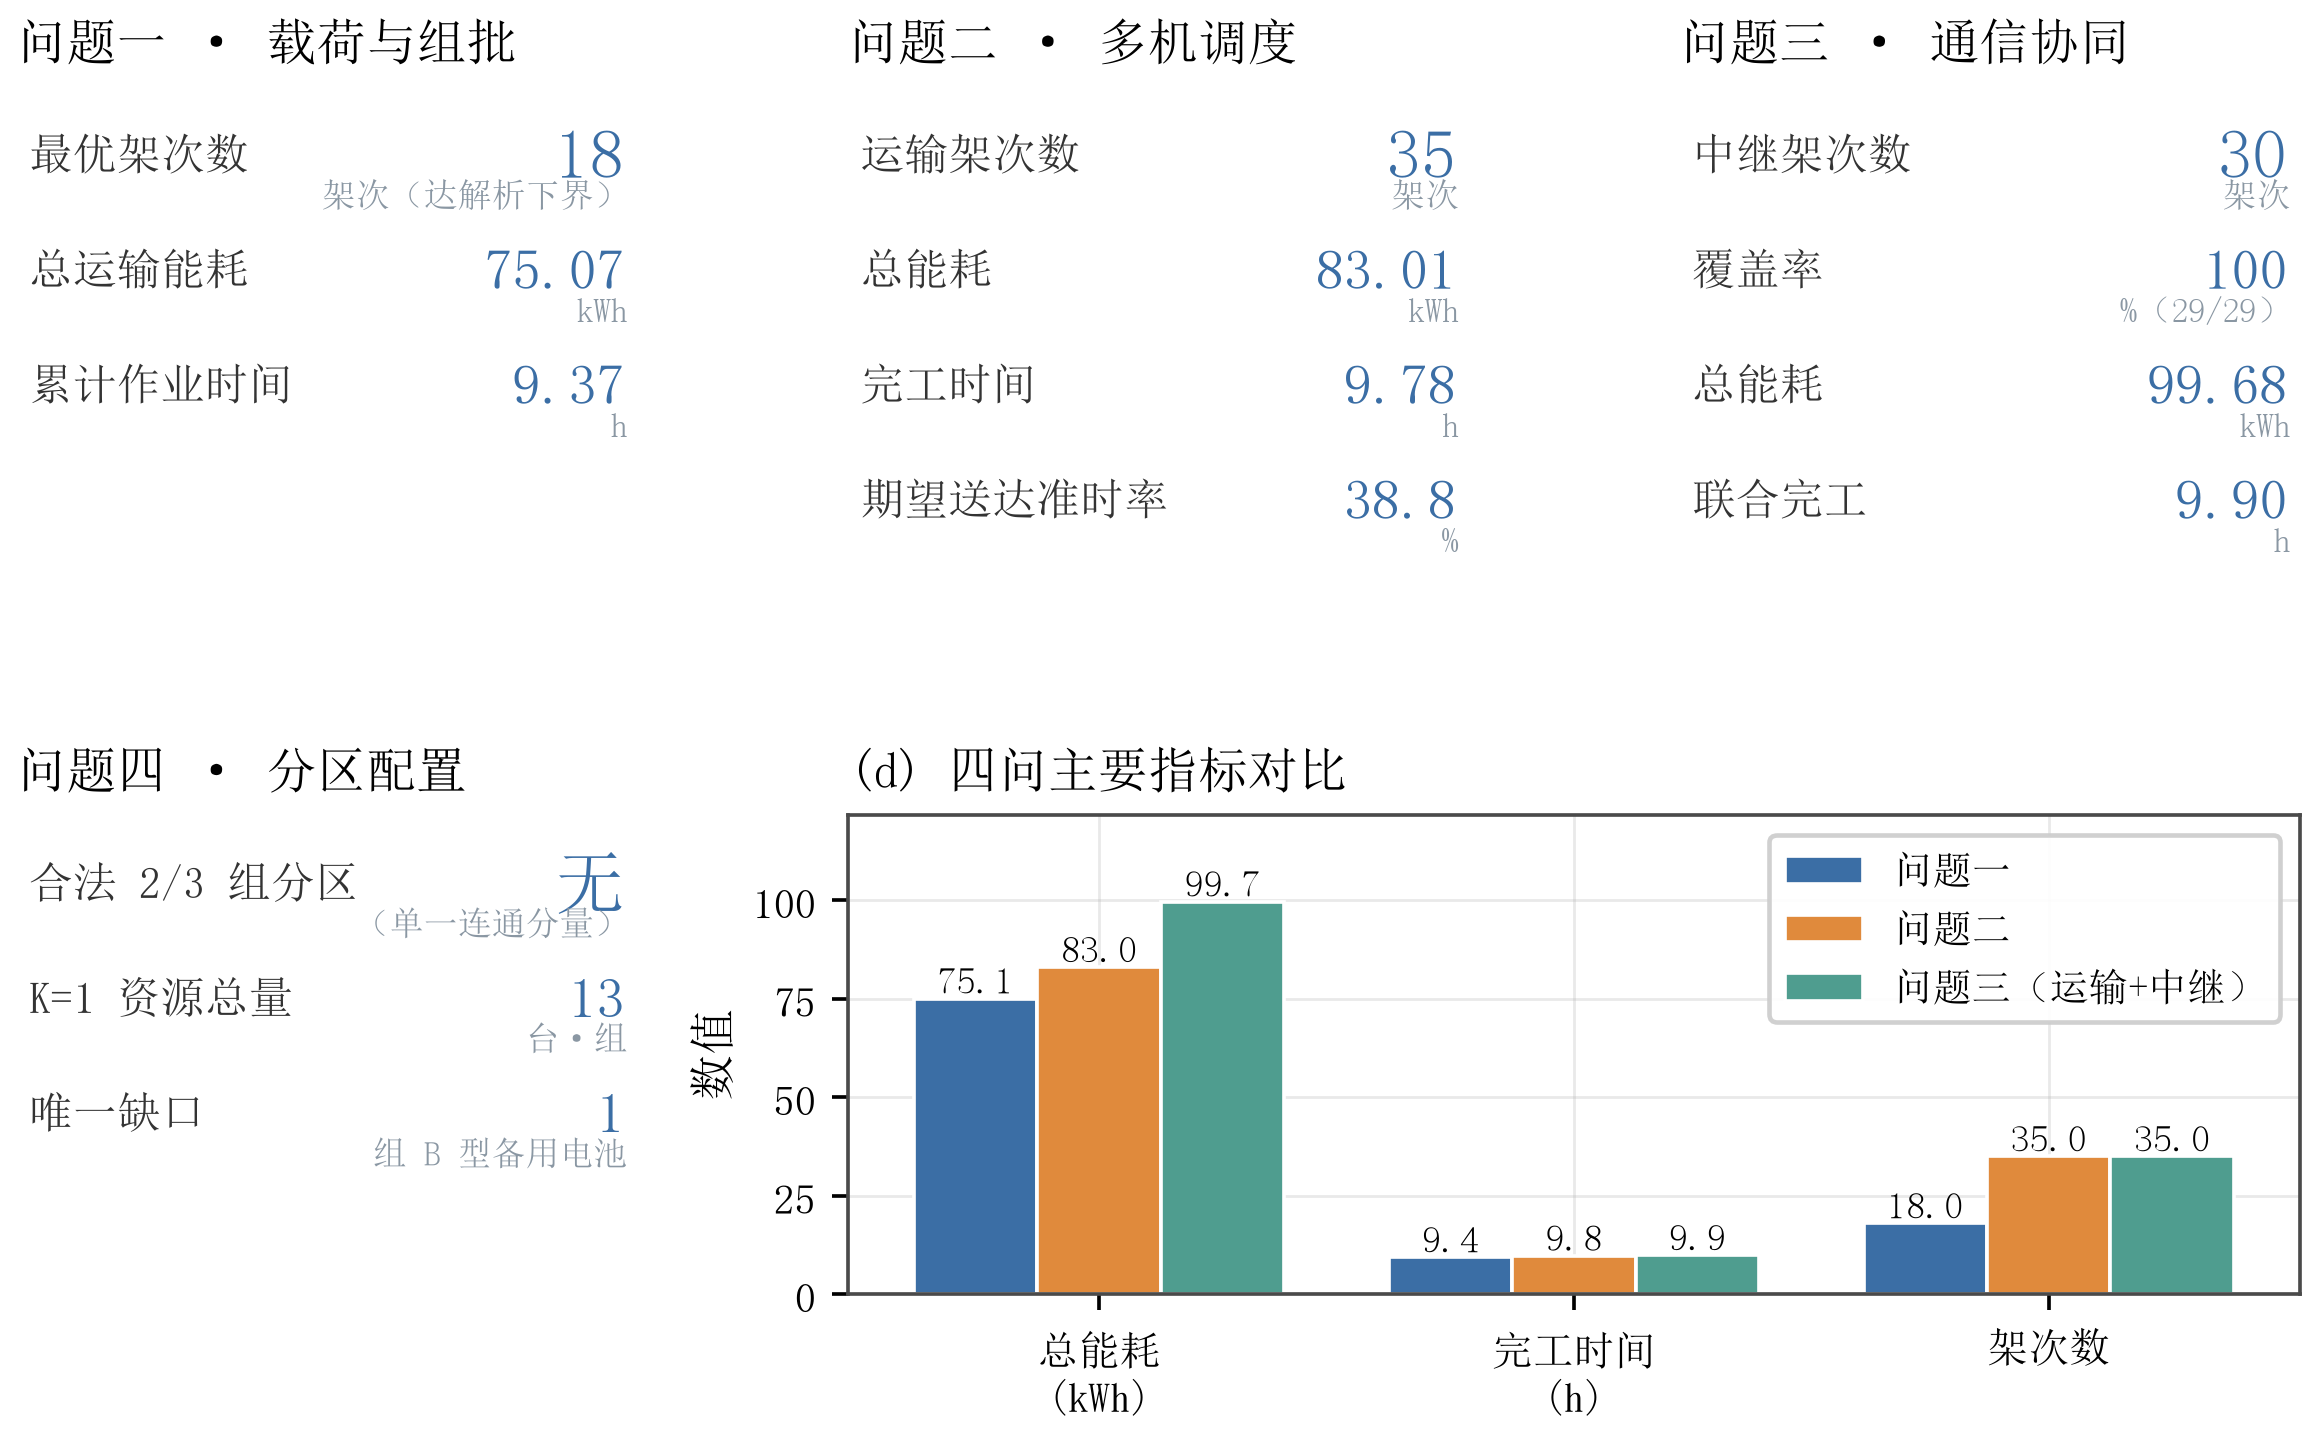
\includegraphics[width=0.98\textwidth]{figures/fig38_summary.png}
	\caption{四问关键指标汇总}
	\label{fig:summary}
\end{figure}

本文的全部数据、程序与图表均可复现，求解脚本按问题分文件组织，图表数据源与结果文件随文附件一并提交。
